\documentclass{acm_proc_article-sp}
\bibliographystyle{unsrt}

\begin{document}

\title{Cellular Automata for Artificial Life Games}
\numberofauthors{2}
\author{
% 1st. author
\alignauthor
Alan S. Wang\\
       \affaddr{Department of Bioengineering}\\
       \affaddr{University of California}\\
       \affaddr{California, Berkeley}\\
% 2nd. author
\alignauthor
Ian Holmes\\
       \affaddr{Department of Bioengineering}\\
       \affaddr{University of California}\\
       \affaddr{California, Berkeley}\\
       \email{ihh@berkeley.edu}
}
\date{30 November, 2013}

\maketitle
\begin{abstract}
A turn-based multiplayer game platform has been developed for mobile devices.
The platform uses cellular automata to implement models
from condensed-matter physics, mathematical biology,
and the computational study of artificial life.
\end{abstract}

% A category with the (minimum) three required fields
%\category{H.4}{Information Systems Applications}{Miscellaneous}
%A category including the fourth, optional field follows...
%\category{D.2.8}{Software Engineering}{Metrics}[complexity measures, performance measures]


\section{Introduction}

Goal: 
build simulation game for mobile devices,
set in a persistent, multiplayer, computationally-dense world
using cellular automata ({\em CA}),
featuring models from
condensed-matter physics,
mathematical biology,
 and
the computational study of Artificial Life ({\em A-Life})

Progress report, describing general structure of platform,
and several models from stochastic biophysics
including simulations of polymer and RNA folding kinetics.

\subsection{Cellular Automata}

CA as a platform for stochastic condensed-matter physics and biophysics
\cite{Schiff2007}

CA as a general platform for games
\cite{SimCity,DwarfFortress,Minecraft}
and electronic toys or art \cite{RuckerCAPOW,PowderToy}

\subsection{Artificial Life Models}

Electronic
\cite{VonNeumannBook,Wireworld}

Biological
\cite{ConwaysLife,Langton1986}

Kinematic
\cite{Stevens2011}

\subsection{Molecular Evolution Models}

RNA World
\cite{Woese1967}

Synthetic RNA World
\cite{PaulJoyce2002}

RNA ALife
\cite{journals/alife/Schuster94}

RNA Folding on Lattice
\cite{LeoniVanderzande2003,JostEveraers2010,ZaraPretti2007,GillespieMayneJiang2009}

Protein folding on the lattice. HP model \cite{Dill1985,PandeRokhsar1999}

\section{Simulation}

\subsection{Virtual Machine}

Low-level (machine code):
state machines.

Addressing: local neighborhood.
Memory structure: bitfields. Fixed amount of dynamic storage, 16 bits given over to a type field that selects from a global program.
Remaining dynamic storage 48 bits, plus effectively unlimited read-only global storage.

Instruction set that minimally generalizes the concept of the lookup table, to facilitate partial matching of neighborhoods:
load-add-store, load-switch, load-compare, random-branch.
(Load and Store allow bitfield access.)

Control flow: goto, no loops, no gosub. Program is a Directed Acyclic Graph (DAG) of finite maximum length.
Facilitates analysis and prediction of resource usage---requirements for player-uploaded programs.

In principle do not need indirect addressing: can explicitly enumerate all cases.
In practice, useful to allow some indirect addressing, to reduce program sizes.

Low-level (assembly language):
Scheme. Generates (assembles) instructions for state machine.
Large built-in library for replicating patterns over Moore or von Neumann neighborhoods,
implementing reaction-diffusion models, implementing turtle-type agents, etc.

Observations on model scaling:
Lookup/modify, no indirect addressing (closest thing to state tables): 2.3Mb.
Only 52k gzipped (still vicious to expand).
With indirect addressing: down to 127k (gzipped: 3k).
Scheme generator is 5k (gzipped: 1k).


Higher-level (path-finding, goal-satisfaction, and other agent-level scripting):
Scheme. S-expression dynamic storage associated with each cell.

Low-level state machine can move or destroy higher-level S-expression storage, but not copy or increase it.
The stringent constraints on the low-level state machine mean that it is safe to open up some of the space of programs to the player,
while maintaining strong performance guarantees on the worst-case simulation rate.

Board:
Cubic lattice.
Square slab, $S \times S \times D$.


\subsection{Polymers}

Doi-Edwards theory \cite{DoiEdwards1988}

As shown in Figure~\ref{fig:polymer}.

\begin{figure}
\fbox{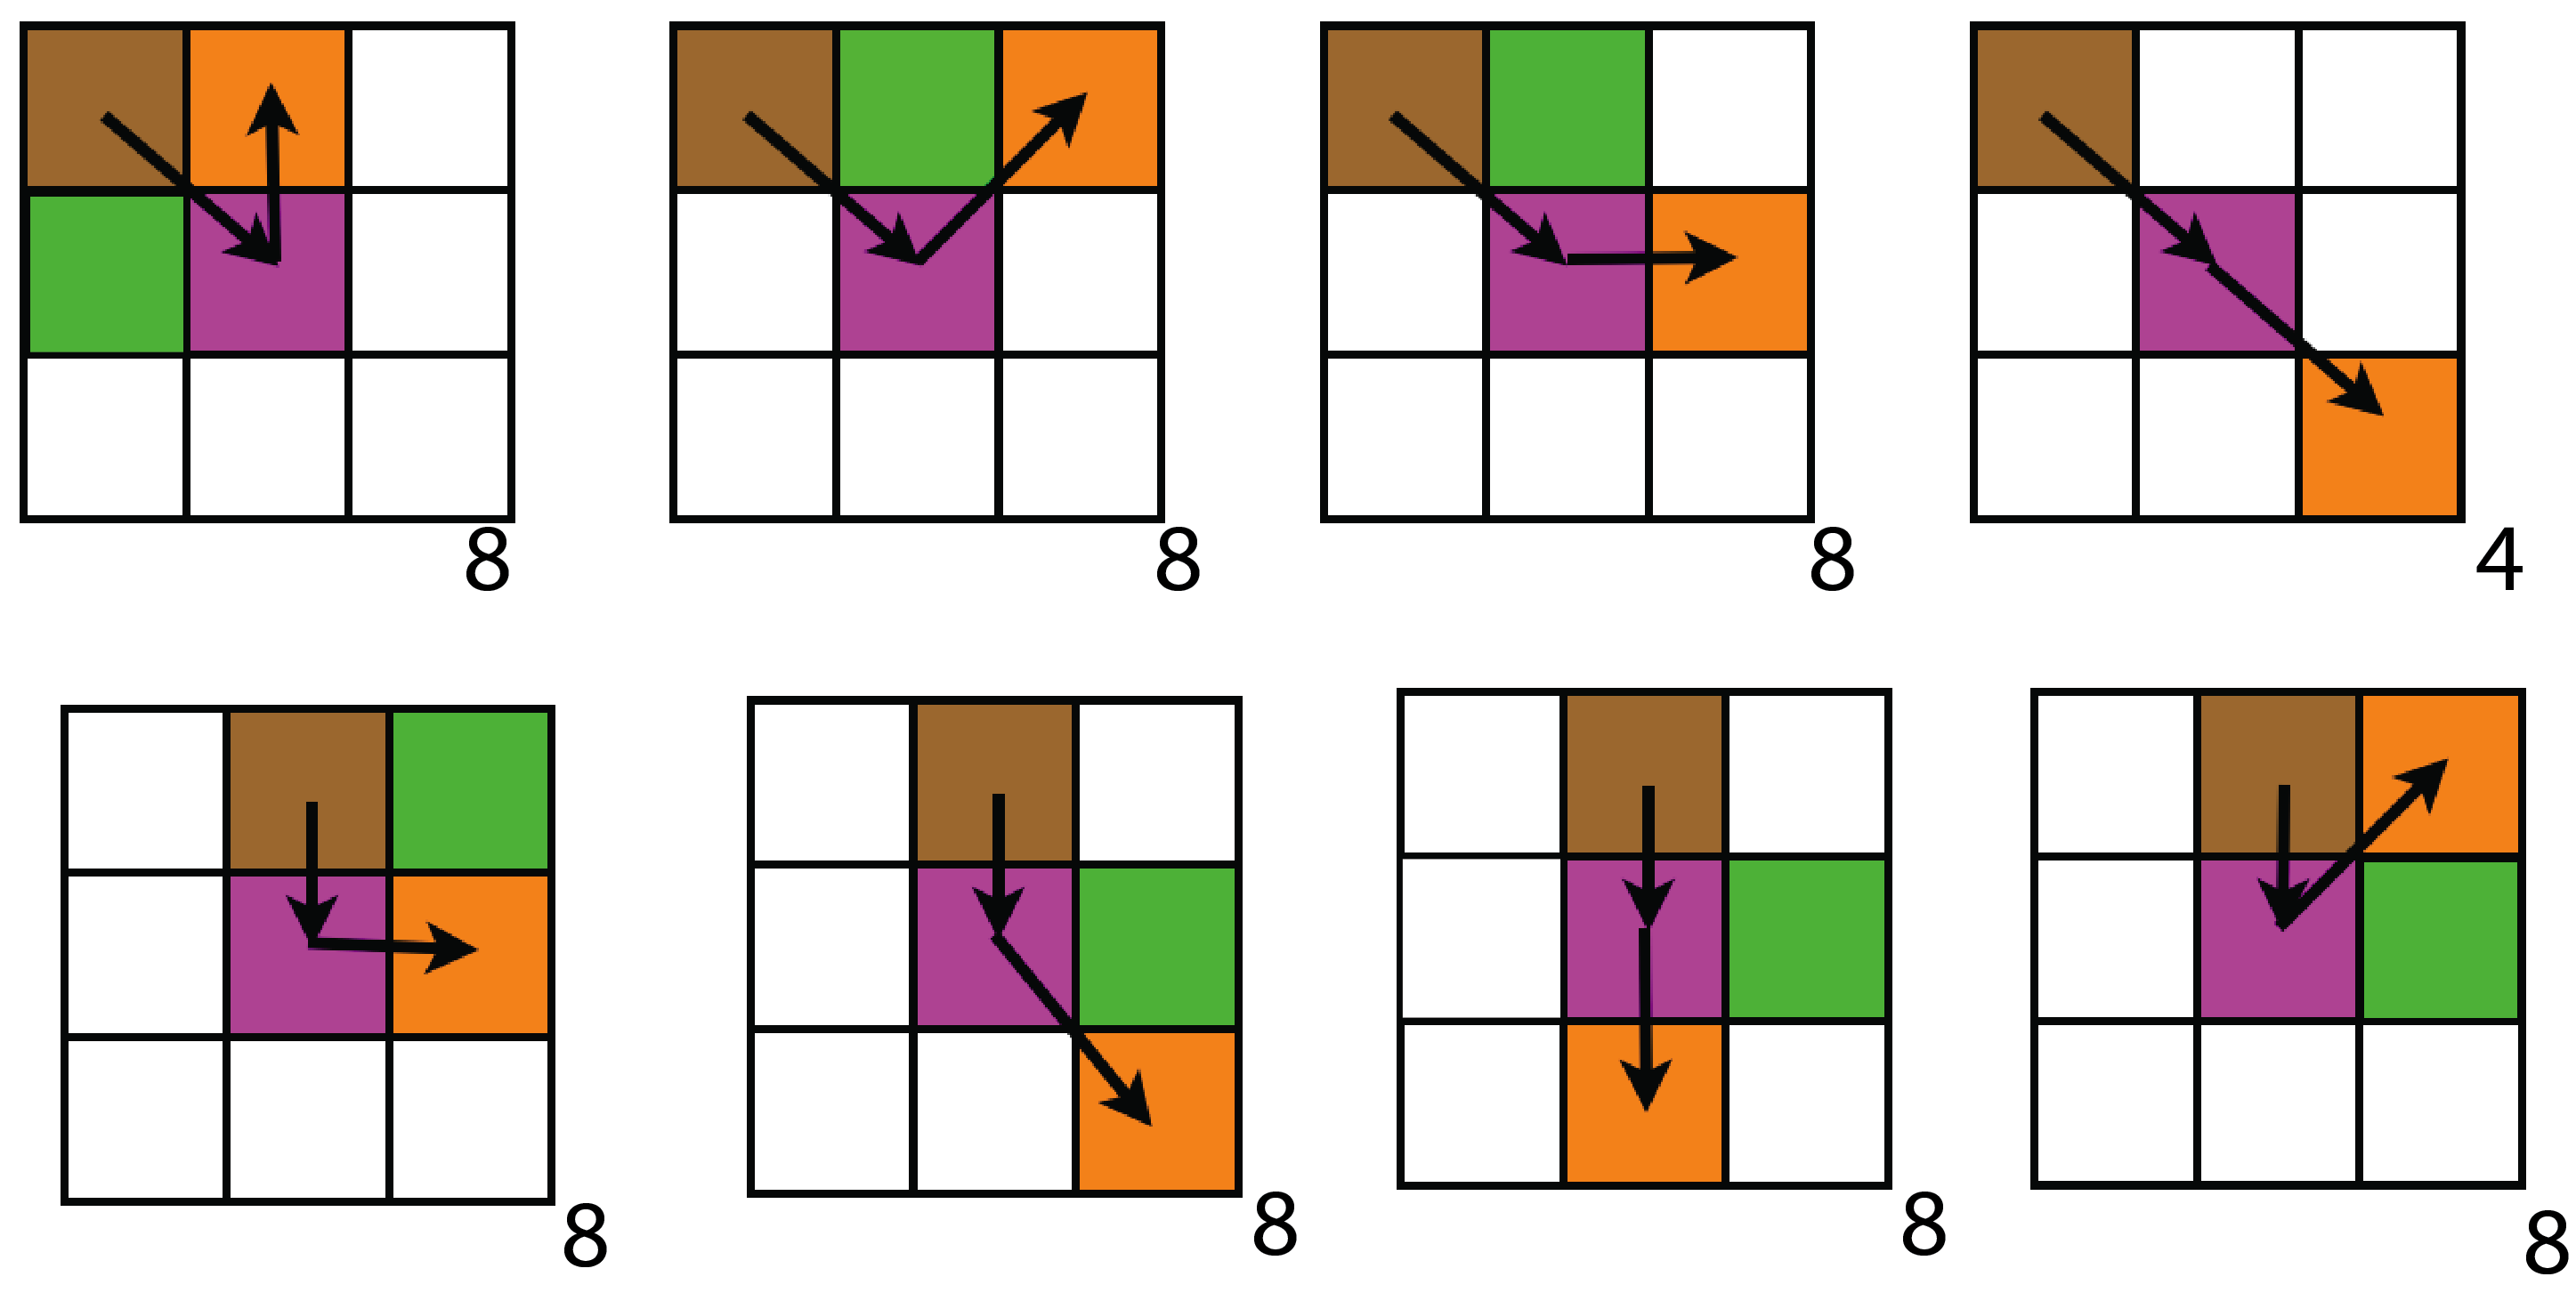
\includegraphics[width=\columnwidth]{Polymer.png}}
\caption{
\label{fig:polymer}
A few cases in the explicit automata-theoretic enumeration of polymer diffusion on the square lattice.
}
\end{figure}


\subsection{RNA Folding}

RNA on a lattice \cite{LeoniVanderzande2003,JostEveraers2010,ZaraPretti2007,GillespieMayneJiang2009}


As shown in Figure~\ref{fig:rna}.

\begin{figure}
\fbox{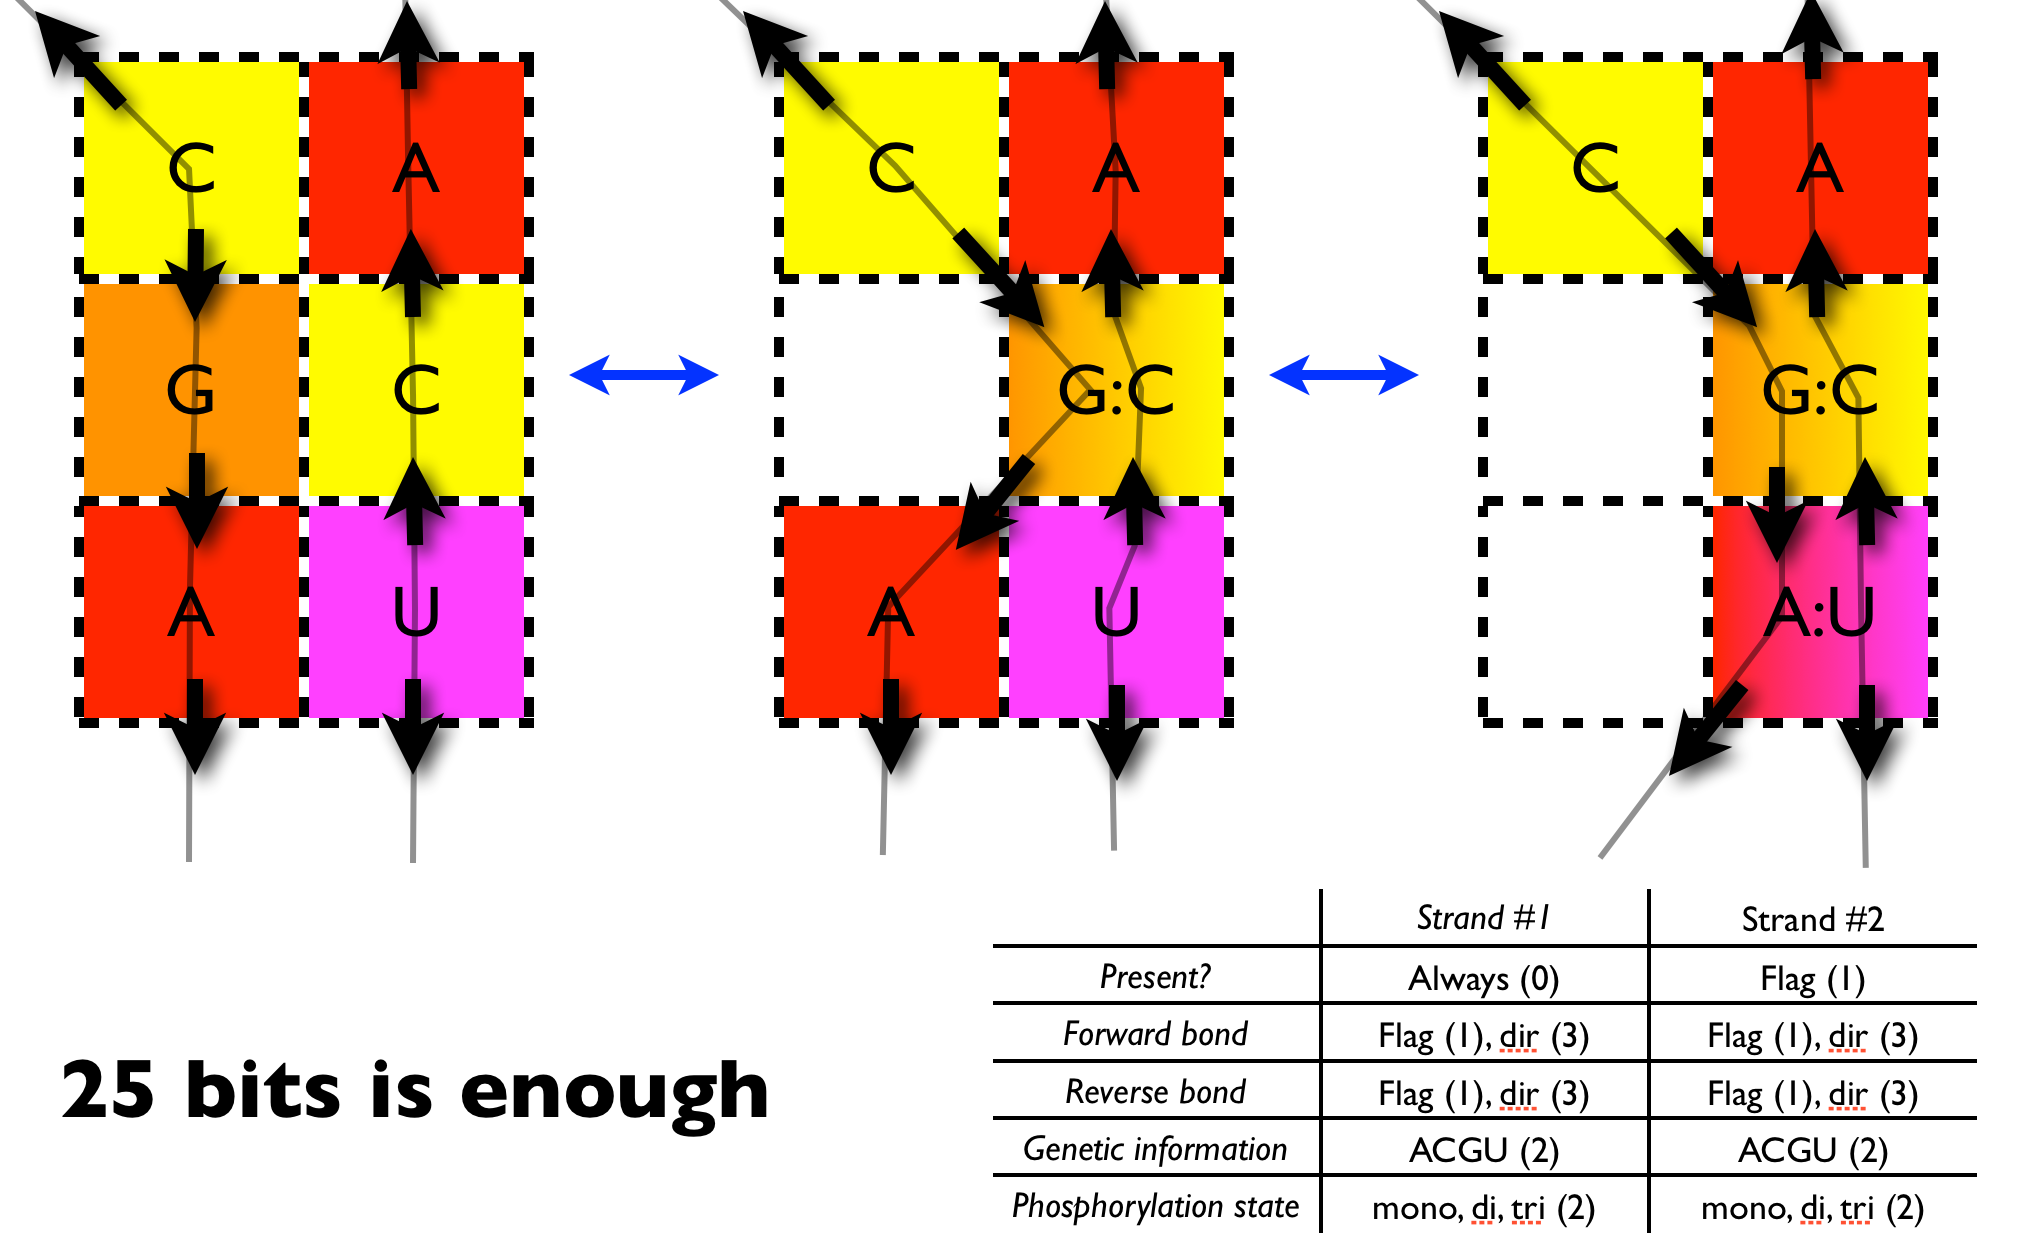
\includegraphics[width=\columnwidth]{RNA.png}}
\caption{
\label{fig:rna}
A sample case in the explicit automata-theoretic enumeration of RNA folding on the square lattice.
}
\end{figure}

\subsection{Agent Patterns}

Tumble-run: {\em E.coli}.
\cite{RosserEtAl2013}

%Sudoku ant: push obstacle a random number of blocks before changing direction.
%\cite{AntBehaviorNature}

Reaction-diffusion.
Directed diffusion.
Diffusion-limited aggregation.
\cite{DLA}

Two-dimensional square-lattice Ising model \cite{Onsager1944}.

Lotka-Volterra (predator-prey) \cite{LotkaVolterra,SpatialLotkaVolterra}.
Rock-paper-scissors games in ecology \cite{Tainaka2000}.

Ecosystem balancing and stability of food webs \cite{quince2005topological}.

Population dynamics and spatial versions of the Wright-Fisher model \cite{MathiesonMcVean2013}.

\section{Game Design}

\subsection{Basic Play}

Terraforming simulation.
Isometric PAINT with live pixels.

Game goal: maintain dynamic equilibrium between three RPS species within a vesicle.

\subsection{Network Play}

Multiplayer implementation: RESTful server \cite{rest}.
Post lock, check board out/in.

Time-limited turns, minimum time between turns, max tool recharge per day.

Multiplayer goal: keep your population alive under attack.

Earn money from your population.

Client: log in/out, browse worlds, pick a world, select terraforming tools...

\subsection{Creating New Tools}

Planned: HTML controls.

Spend money creating and using new reaction-diffusion particles and spray-tools.

\subsection{Implementation}

Gnu C, libXML, GDataXML, ChibiScheme, XCode, Catalyst (Perl).

\section{Discussion}

Work in progress.

\subsection{Acknowledgements}

Many thanks are due Alex Shinn, Richard Evans, Michael Mateas, Sean Eddy, Gerald Joyce, Chris Quince,
and Rudy Rucker for help and inspiration.


\bibliography{pzpaper}

\balancecolumns
% That's all folks!
\end{document}
